\documentclass{llncs}
\usepackage[noend]{algpseudocode}
\usepackage{subcaption}
\usepackage{subfig} 
\usepackage{usual}
\usepackage{amsmath}
\usepackage{graphicx}
\usepackage{eulervm}
\usepackage{fontenc}
\pagenumbering{alph}

\usepackage[rflt]{floatflt}
%\pagestyle{plain}
%
\begin{document}
\title{\vskip -10pt}

\maketitle 

\section{Model of preferences}
In this section, we present our model of preferences on which the negotiation is based.
\subsection{Preferences}
\par We allows the conversational agent to have preferences also to be able to understand user preferences. We assume that the agent expresses its preferences on a defined object based on one or multiple criteria.   
 \begin{itemize}
 \item Objects $O$ : Set of all possible objects of negotiation. For example, negotiate to find at which restaurant have dinner. Note that $O$ is a set of instances of the same type (restaurants in our example):
  \\ $O=\{Ginza, LeDragonD'Or,  Venezzia, \ldots\}$
 \item Criteria $C$: set of criteria or features of preferences on objects. For example, we assume that we can choose a restaurant based on one or several of the following criteria = \{cuisine, ambiance, price, location\}. Each criterion has its domain of values that we note: $\forall c \in C$, $D_{c}$ is its domain. For example $D_{cuisine} = \{chineese, italian\}$.

 \item $\forall o \in O, \forall c \in C$, we define $v(c,o) \in D_{c}$ as the objective value of the criterion $c$ attributed to the object $o$. For example, Ginza is an expensive Japanese restaurant. Thus $v(price, Ginza) = expensive$ and $(cuisine, Ginza) = japanese$. 
 
 \item Lets now define interlocutor's preferences.[Rephrase] $\forall agent_{i}$ that has to define its preference for an object, for example a restaurant.
 \begin{itemize}
 \item Preferences on criteria of quality related to the object: $Pref_{i}^C (X,Y) $ is a total ordered set of criteria. For example, $ Pref_{i}^{restaurant} (cuisine,price)$ means that the criterion of cuisine is more important for the $agent_{i}$  than the price to choose a restaurant. 
 \item Once the criteria is defined, the $agent_{i}$ defines his preferences on the domain of this criteria. Thus, $\forall v_{1} , v_{2} \in D_{C}$, the agent has a  partially ordered preferences on these values noted $Pref_{i}^C (v_{1}, v_{2})$  which can be represented as $v_{1}>_{C} v_{2}$ . For example, $agent_{i}:  Pref_{i}^{cuisine} (Japanese , Chinese)$ , means that  $agent_{i}$ prefers the Japanese cuisine over the Chinese. $v_{1} $ and $ v_{2}$ can take other values as presented : 
 \subitem $Pref_{i}^C (v_{1}, *)$ means that $agent_{i}$ prefers the most $v_{1}$. 
 \subitem $Pref_{i}^C (*,v_{2})$ means that $agent_{i}$ doesn't like  $v_{2}$. 
 \subitem $Pref_{i}^C (*,*)$ means that $agent_{i}$ has no preference on $C$. 
 \item The last step consists in defining the agent preferences on the object "restaurant". [Rephrase]Based on what we defined above, we conclude that defining a preference on an object is a multi criteria decision \cite{figueira2005multiple}. We denote a function of decision  $Dec$ such that $\forall o_{1}, o_{2} \in O x O, Dec$ define an order of preference on these objects where  $\{o_{1}\prec o_{2}, o_{1} \succ o_{2}, o_{1} \approx o_{2}\}$.
 \end{itemize} 
 \end{itemize}
 \subsubsection{Decision function}
 	Here represent the function of decision.
 \subsection{Mental state}
 To be able to negotiate, the agent need a formal representation of its environment namely, its preferences, the user preferences and the  knowledge shared during the conversation. 
\subsubsection{Shared knowledge}
 
During dialogue, interlocutors  negotiate  about an object and its criteria that define it. The final decision is to select an object (\emph{e.g.} let's go to Ginza), but during the negotiation, agents can also propose values for criteria (\emph{e.g.} let's go to a Japanese restaurant). To represent these elements of negotiation, we use the following notations:
 \begin{itemize}
	 \item Propose an object: 
	 	\subitem Let $P_o$ be the set of proposed objects during the dialogue where $Propo_i(o)$ means that $agent_i$ proposed the object $o$ and therefore $o\in P_o$.
	 	\subitem Let  $R_o$  be the set of rejected objects $o\in O$ such as $Rej_i(o)$ means that the $o$ has been rejected during the dialogue. Thus $O \in R_o$
	 	\subitem $\theta_{o} = O-\{ P_o, R_o\}$ is the set of objects that don't have been discussed yet, and $o=max_i(\theta_{o})$ is the most preferred object of $agent_i$ that has not been reject. Thus, $choice_i= o$.
	\item In the same idea, proposing a criterion is modeled follows:   
		\subitem Let $C$ be the set of criteria $c \in C$ and their domain of values $D_c$. Thus, proposing a value $v$ for a criterion $c$ is defined $Prop_i(c,v)$. 
		\subitem $P_c$ can be defined in two manners: 1)- as a set of tuples that represent all the criteria and their values that were proposed in the dialogue. Thus $(c,v) \in P_c$. 2)- we define a set for each criterion $c$. Thus $P_c$ contains all the proposed values for the criterion $c$ during the dialogue.
		\subitem $R_c$ is the set of rejected values for criteria in the dialogue (The same representation than $P_c$ with the same deal of representation).
		\subitem  $\theta_{c} = D_c - \{P_c, R_c\}$ is the set of non proposed criteria in the dialogue, or the values that were not proposed for a certain criterion. thus 
		%where $FDec(c,*) $ (\textit{i.e} $c$ has no defined value). 
   
   \item $Dec(o)$ represents the fact that the final decision is to choose object $o$ (eg: the Ginza restaurant)
   \item $Dec(c,v)$ represents the fact that the final decision must choose an object that has value $v$ for criteria $c$ (eg: a silent restaurant)
 \end{itemize}


% ici axiomes:
% - axiome de coopération
% - axiome de propositions/décision
% $B_i I_j Dec(x) et _cette décision est compatible avec mes prefs_ => I_i Dec(x)
% ou alors à quel moment je rajoute un I_i Dec dans ma base pour faire un propose ?

\subsubsection{Utterances semantic}
Agents communicates using utterances that encapsulate the message. After each communicated utterance, agents will update their beliefs about the preferences of the other agent. Therefore an utterance is communicated to a need to update a belief. In the following, we suppose that $agent_{i}$ is the speaker and $agent_{j}$ is the hearer. As messages are actions, they are defined with precondition and effects on the belief. The preconditions are all optional, because the message selection depends first on the agent strategy of conversation. However, defining preconditions allow us to do inferences in order to know the reasons that make the agent choose this action. For example, if the agent changes the subject of discussion and talks about Chinese food, then we can conclude that the agent is dominant enough to lead the dialogue and change the subject of discussion. In addition, the effects are symmetric, we only represent the  agent's belief about its preferences and user preferences. We cannot represent the user belief, we can only represent the agent perception of the user belief. For example, we situate our perception form the agent point of view. Suppose that the agent states that he likes Chinese food.  We can imagine that the reasons (precondition) that lead him  to state its preferences was that the agent believed that the user didn't know the agent preference and the agent also had the intention to inform the user about its preferences. The effect of the statement is that now the agent believes that the user knows that he likes Chinese food. 

In the following, we will be presenting  the utterances of dialogue and their effects on the agent belief in the case where the agent is either the hearer (\textit{i.e} Agent = $agent_i$) or  the listener(\textit{i.e} Agent = $agent_j$). We specify that the effects of the speaker (i)  are always of the form $B_i Effects(j)$, but in some situation this does not bring any useful knowledge for the reactive planer so we ignore it. In addition, utterances update only the belief of the agent about preferences but at any case utterances change the values of preferences in the dialogue (no action can have any effect on the preferences of the interlocutor). 

%Par exemple, pour le statePref, on peut considérer 2 situations:
%- i=humain, j=agent: si l'humain me dit qu'il aime le chinois, je peux 1) déduire que, probablement, il croyait que je ne le savais pas, 2) il avait l'intention que je le sache (obtenu à partir des préconditions) et 3) qu'il croit que maintenant je le sais et surtout, que moi, maintenant, je le sais: je l'ajoute dans ma base.
%- i=agent, j=humain: si je dis à l'humain que j'aime le chinois, c'est parce que je pensais qu'il ne le savait pas et j'avais envie qu'il le sache. Je ne peux rien dire sur ses croyances mais maintenant, je crois qu'il le sait: j'ajoute cette croyance dans ma base

 \begin{itemize}
 \item State.Preference(\textit{$P_{1}, P_{2}$}) : I prefer $P_{1}$ over $P_{2}$.
	 \subitem Preconditions(i):  $ B_{i} U_{j} Pref_{i}(P_{1}, P_{2}), I_{i} B_{j} Pref_{i}(P_{1}, P_{2})$
	 \subitem Effects(j): $ B_{j} Pref_{i}(P_{1}, P_{2})$
	 \subitem Effects(i): $ B_i Effect(j)$ (not really useful for the agent to know that the user knows its preferences ?)
	 \\ We define two variant valuations on stating preferences as follows: 
	 \subitem State.Preference(\textit{$P_{i}, *$}): I prefer the most $P_{i}$.
	 \subitem State.Preference(\textit{$*, P_{i}$}): I don't like /hate $P_{i}$.
	 \subitem Example: State.Preference(\textit{$Pref_{i}^{cuisine} (Japanese , Chinese)$}) : I prefer japanese cuisine over chinese.

 \item Ask.Preference(\textit{$P_{1}, P_{2}$}) : Do you prefer $P_{1}$ to $P_{2}$ ?. 
	  \subitem Preconditions:  $ U_{i} Pref_{j}(P_{1}, P_{2})$ ,  $ I_{i} B_{i} Pref_{j}(P_{1}, P_{2})$
	  \subitem Effects (j):  $B_{j} U_{i} Pref_{j}(P_{1}, P_{2})$ ,  $ B_{j} I_{i} B_{i}Pref_{j}(P_{1}, P_{2})$
	  \subitem Effects(i): $ B_i Effect(j)$ (not really useful for the agent to know that the user knows that the agent wants to know, imho)
	 \\We define two variant valuations as follows: 
	 \subitem Ask.Preference(\textit{$Pref_{j}(P_{1}, *)$}): Do you like $P_{1}$?
	 \subitem Ask.Preference(\textit{$*$}): What do you like ?. This case appear when the speaker has no belief on the hear preferences. 
	 \subitem Example: Ask.Preference$^{cuisine}$(\textit{$Japanese , Chinese$}) : Do you prefer japanese cuisine or chinese?

 \item Ask.Object(): Which "Object" do you want to choose ? For example we consider Object = Restaurant. Note that Ask.Object has no content. Since we consider a single-object negotiation, the participants have to choose one single element in $O$. The semantic of the utterance Ask.Object means that the sender asks the hearer to propose an instance $o\in O$.
	\subitem Preconditions:  $ U_{i} Pref_{j}(*,*)$ ,  $ I_{i} B_{i} Pref_{j}(*,*)$
  	\subitem Effects (j):  $B_{j} U_{i} Pref_{j}(*, *)$ ,  $ B_{j} I_{i} B_{i}Pref_{j}(*,*)$
 
 \item Propose.Criteria(\textit{V(criteria, value)}): I think that \textit{value}  would be great. 
	  \subitem Preconditions:  $ I_{i} Prop_i(criteria, value) $
	  \subitem Effects:  $B_{j} I_{i} Prop_i(criteria, value)$
	  \subitem Example: Propose.Preference(\textit{$V(cuisine,Japanese)$}) : I want to taste japanese food.

 \item Accept.Criteria(\textit{V(criteria, value)}): Okay, let's choose \textit{value}. After receiving a propose utterance from the $agent_{j}$,  $agent_{i}$ might accept the proposal.
   \subitem Preconditions: $ B_i Prop_j (V(criteria, value))$
   \subitem Effects:  $B_{i,j} Pref_{i,j}(V(criteria, value))$
   
 \item Reject.Criteria(\textit{V(criteria, value)}): Sorry, I would choice something else.
    \subitem Preconditions: $ B_i Prop_j (V(criteria, value))$
    \subitem Effects:  $B_{j} \neg  Pref_{i}(V(criteria, value))$
 
  \item Propose.Object(\textit{object}): I think that \textit{object} would be great.
  \subitem Preconditions:  $ I_{i} Prop_{j}(object)$
  
  \subitem Effects:  $B_{j} I_{i} Prop_{j}(object)$ ,  $ B_{j} Pref_{i}(object)$  
  \item Accept.Object(\textit{object}): Okay, let's choose \textit{value}.
     \subitem Preconditions: $ B_i Prop_j (object)$
     \subitem Effects:  $B_{i,j} Pref_{i,j}(object)$ 
  
  \item Reject.Object(\textit{object}): Sorry, I would choice something else.
     \subitem Preconditions: $ B_i Prop_j (object)$
      \subitem Effects:  $B_{j} \neg  Pref_{i}(object)$
 \end{itemize} 


 

\section{Ideas on multi criteria decision}
The questions that came when I was writing the formal model are the following: 
\begin{enumerate}
	\item When the agent decides to send a \emph{Propose. Object} utterance ?
	\item Based on which decision function should the agent propose an object ?
\end{enumerate}

\subsection{HTN structure for actions and messages}
My first proposition to answer the first question is to use the HTN structure for that. Assume that the task of choosing a restaurant is modeled as represented in the  \fig{tree}. In addition, these tasks are defined with a grounding script in which a decision function (see section \ref{DF}) is called to define which Object/Criterion send with the message. 

\begin{figure}[b]
	\centerline{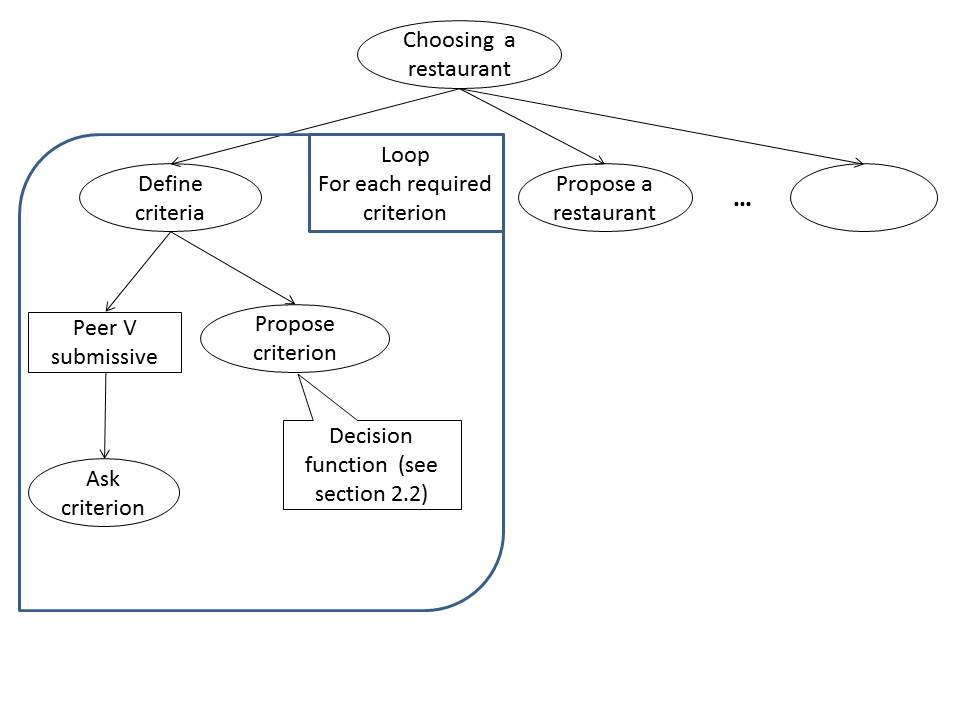
\includegraphics[width=3in]{figs/dialogue_tree}}
	\vskip 8pt
	\defig{tree}{Example pf an HTN modeling to choose a restaurant}
\end{figure}


\subsection{Decision function} \label{DF}
In the context of multi criteria problems, decision making cannot be done without incorporating preferences [add reference]. However, in social interaction, decision makers have to take in account the preferences of the other interlocutors in addition to their preferences, because their choice affect them directly. This field is called social decision. In addition to preferences, we take in account the agent representation of the relationship. Therefore, if the agent is peer or submissive, he'll decide regarding to the user preferences( the ask criteria task). However, a dominant agent is self-interest and will escape this task and focus more on its preferences. 
\subsection{Weighted some model}
\par Therefore, one obvious proposition would be to use the Weighted sum model where the decision function is calculated as follow:

\[Dec(o) = \sum_{j=1}^{n} w_j (c_j,v).\] 
 First, we define preferences on criteria, we assume that the agent has an ordered list of criteria, and we will use  conversation to lean the user preferences on criteria and their (ex: type of cuisine, location .. ). Second, we will define weights on these criteria depending on the preferences (The more the criterion is preferred the more is weighted). Here come the notion of relationship in our decision, the weight of criteria is affected by the relationship, for example a dominant person will weight more her preferences while a interlocutors in peer relation will give equivalent weights to their preferences.  This function can also be used to calculate the acceptability of a proposal that the agent receive, as represented bellow where $S$ represent an acceptability threshold fixed depending on the nature of the relationship.
  \[ Acceptable(o) =
 \begin{cases}
    Dec(o) > S & \quad \text{return Yes }\\
  \text{Otherwise} & \quad \text{return No}\\
 \end{cases}
 \]
 
 \begin{figure}
 	\centerline{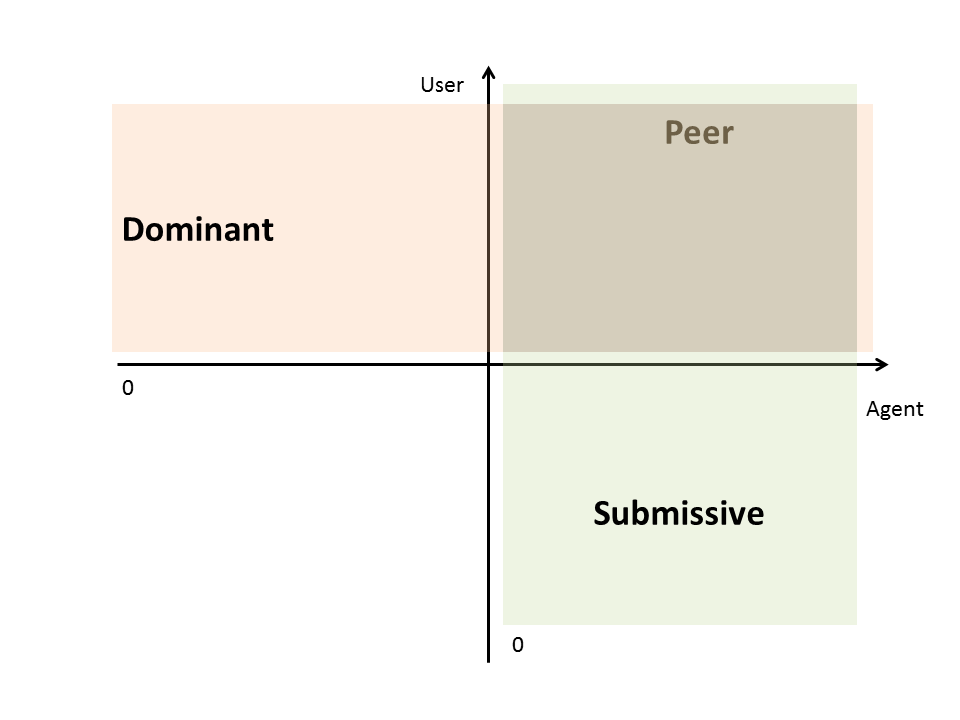
\includegraphics[width=3in]{figs/multiCriteria}}
 	\vskip 8pt
 	\defig{tree}{Domain of decision for the different relations}
 \end{figure}
\subsubsection{Limits of this approach}
\begin{itemize}
\item Different calculation scales of criteria can compromise the comparison of objects. 
\item Define weights that allows optimal solutions. 
\item Calculation under uncertainty: in some cases we ignore the preference of the user on some criteria. 
\end{itemize}
\noindent 
\vskip 4pt
\bibliographystyle{plain}
\bibliography{abbrevs,Library}
\end{document}
